%!TEX TS-program = xelatex
%!TEX options = -aux-directory=Debug -shell-escape -file-line-error -interaction=nonstopmode -halt-on-error -synctex=1 "%DOC%"
\documentclass{article}
\input{LaTeX-Submodule/template.tex}

% Additional packages & macros
\DeclareMathOperator{\grad}{grad}
\DeclareMathOperator{\divergence}{div}
\DeclareMathOperator{\curl}{curl}

% Header and footer
\newcommand{\unitName}{Electrical Engineering Mathematics}
\newcommand{\unitTime}{Semester 1, 2024}
\newcommand{\unitCoordinator}{Prof Scott McCue}
\newcommand{\documentAuthors}{Tarang Janawalkar}

\fancyhead[L]{\unitName}
\fancyhead[R]{\leftmark}
\fancyfoot[C]{\thepage}

% Copyright
\usepackage[
    type={CC},
    modifier={by-nc-sa},
    version={4.0},
    imagewidth={5em},
    hyphenation={raggedright}
]{doclicense}

\date{}

\begin{document}
%
\begin{titlepage}
    \vspace*{\fill}
    \begin{center}
        \LARGE{\textbf{\unitName}} \\[0.1in]
        \normalsize{\unitTime} \\[0.2in]
        \normalsize\textit{\unitCoordinator} \\[0.2in]
        \documentAuthors
    \end{center}
    \vspace*{\fill}
    \doclicenseThis
    \thispagestyle{empty}
\end{titlepage}
\newpage
%
\tableofcontents
\newpage
%
\part{Infinite Series}
\section{Sequences and Series}
\subsection{Sequences}
A sequence is an \textbf{ordered list} of numbers
\begin{equation*}
    a_1, \: a_2, \: a_3, \: \ldots, \: a_n, \: \ldots
\end{equation*}
denoted \({\left\{ a_n \right\}}_{n=1}^{\infty}\), where
\(n\) is the index of the sequence.
A sequence can be \textbf{finite} or \textbf{infinite}.
\subsection{Limits of Sequences}
An infinite sequence \(\left\{ a_n \right\}\) has a limit \(L\) if
\(a_n\) approaches \(L\) as \(n\) approaches infinity:
\begin{equation*}
    \lim_{n \to \infty} a_n = L
\end{equation*}
If such a limit exists, the sequence \textbf{converges} to \(L\).
Otherwise, the sequence \textbf{diverges}. Sequences that oscillate
between two or more values do not have a limit.
\subsection{Series}
Given a sequence \(\left\{ a_n \right\}\), we can construct a sequence
of \textbf{partial sums},
\begin{equation*}
    s_n = a_1 + a_2 + \cdots + a_n
\end{equation*}
denoted \(\left\{ s_n \right\}\), such that when \(\left\{ s_n \right\}\)
converges to a finite limit \(L\), that is,
\begin{equation*}
    \lim_{n \to \infty} s_n = L
\end{equation*}
the \textbf{infinite series} \(\sum_{n=1}^{\infty} a_n\) converges to \(L\).
Otherwise, the series \(\sum_{n=1}^{\infty} a_n\) diverges.
\subsubsection{Common Series}
Below are a list of common series that converge to a finite limit:
\begin{itemize}
    \item \textbf{Geometric Series}: A sum of the geometric progression
          \begin{equation*}
              \sum_{n=0}^{\infty} a r^n
          \end{equation*}
          converges when \(\abs*{r} < 1\), and diverges otherwise. When
          \(\abs*{r} < 1\),
          \begin{equation*}
              \sum_{n=0}^{\infty} a r^n = \frac{a}{1 - r}
          \end{equation*}
    \item \textbf{Harmonic Series}: A sum of the reciprocals of natural numbers
          \begin{equation*}
              \sum_{n=1}^{\infty} \frac{1}{n}
          \end{equation*}
          always diverges.
    \item \textbf{\(p\)-Series}: A sum of the reciprocals of \(p\)-powers of
          natural numbers
          \begin{equation*}
              \sum_{n=1}^{\infty} \frac{1}{n^p}
          \end{equation*}
          converges when \(p > 1\), and diverges otherwise. This series is
          closely related to the \textbf{Riemann Zeta Function}, and has
          exact values for even integers \(p\).
\end{itemize}
\subsection{Convergence Tests}
There are several tests to determine the convergence of an infinite
series. Note that these tests do not determine the value of the limit.
\subsubsection{Ratio Test}
Given the infinite series \(\sum_{n=1}^{\infty} a_n\), with
\begin{equation*}
    \rho = \lim_{n \to \infty} \abs*{\frac{a_{n+1}}{a_n}}
\end{equation*}
\begin{enumerate}[label=(\arabic*)]
    \item If \(\rho < 1\), the series converges.
    \item If \(\rho > 1\), the series diverges.
    \item If \(\rho = 1\), the test is inconclusive.
\end{enumerate}
\subsubsection{Alternating Series Test}
Given the infinite series \(\sum_{n=1}^{\infty} {\left( -1
\right)}^{n-1} b_n\), the alternating series converges if the following
conditions are met:
\begin{enumerate}[label=(\arabic*)]
    \item \(b_n > 0\) for all \(n\).
    \item \(b_{n+1} \leqslant b_n\) for all \(n\).
    \item \(\lim_{n \to \infty} b_n = 0\).
\end{enumerate}
\section{Taylor Series}
\subsection{Taylor Polynomials}
A Taylor polynomial is a polynomial that approximates a function near a
point \(x = x_0\). The \(n\)-th order Taylor polynomial of an
\(n\)-times differentiable function \(f\left( x \right)\) near \(x =
x_0\) is given by:
\begin{equation*}
    P_n\left( x \right) = f\left( x_0 \right) + f'\left( x_0 \right) \left( x - x_0 \right) + \frac{f''\left( x_0 \right)}{2!} {\left( x - x_0 \right)}^2 + \cdots + \frac{f^{\left( n \right)}\left( x_0 \right)}{n!} {\left( x - x_0 \right)}^n
\end{equation*}
Using summation notation, this becomes,
\begin{equation*}
    f\left( x \right) \approx P_n\left( x \right) = \sum_{k=0}^{n} \frac{f^{\left( k \right)}\left( x_0 \right)}{k!} {\left( x - x_0 \right)}^k
\end{equation*}
If \(f\) is (\(n+1\))-times differentiable on an interval including
\(x_0\), then the error of this approximation can be bounded by
\begin{equation*}
    R_n\left( x \right) = f\left( x \right) - P_n\left( x \right) = \frac{f^{\left( n+1 \right)}\left( p \right)}{\left( n+1 \right)!} {\left( x - x_0 \right)}^{n+1}
\end{equation*}
for some \(p\) between \(x\) and \(x_0\).
\subsection{The Taylor Series}
The Taylor polynomials can be extended to Taylor series by taking the
limit \(n \to \infty\). The Taylor series of an infinitely
differentiable function \(f\left( x \right)\) near \(x = x_0\) is
defined:
\begin{equation*}
    f\left( x \right) = \sum_{n=0}^{\infty} \frac{f^{\left( n \right)}\left( x_0 \right)}{n!} {\left( x - x_0 \right)}^n
\end{equation*}
When \(x_0 = 0\), the Taylor series is called the \textbf{Maclaurin series}.
\subsection{Convergence of Taylor Series}
The Taylor series is a form of a \textbf{power series}:
\begin{equation*}
    \sum_{n=0}^{\infty} c_n {\left( x - x_0 \right)}^n.
\end{equation*}
A power series may converge in one of three ways:
\begin{enumerate}[label=(\arabic*)]
    \item At a single point \(x = x_0\), with a radius of convergence
          \(R = 0\).
    \item On a finite open interval \(\ointerval{x_0 - R}{x_0 + R}\),
          with a radius of convergence \(R > 0\). The series is not
          guaranteed to converge at the endpoints of this interval.
    \item Everywhere, with a radius of convergence \(R = \infty\).
\end{enumerate}
For elementary functions, the Taylor series converges to the function
everywhere within the radius of convergence.
\subsection{Common Taylor Series}
Below is a list of common Taylor series expansions:
\begin{table}[H]
    \centering
    \begin{tabular}{c c c}
        \toprule
        \textbf{Function}             & \textbf{Taylor Series}                                                                           & \textbf{Convergence}     \\
        \midrule
        \(e^x\)                       & \(\displaystyle\sum_{n=0}^{\infty} \frac{x^n}{n!}\)                                              & \(-\infty < x < \infty\) \\
        \(\sin{\left( x \right)}\)    & \(\displaystyle\sum_{n=0}^{\infty} \frac{{\left( -1 \right)}^n x^{2n+1}}{\left( 2n+1 \right)!}\) & \(-\infty < x < \infty\) \\
        \(\cos{\left( x \right)}\)    & \(\displaystyle\sum_{n=0}^{\infty} \frac{{\left( -1 \right)}^n x^{2n}}{\left( 2n \right)!}\)     & \(-\infty < x < \infty\) \\
        \(\ln{\left( 1 - x \right)}\) & \(\displaystyle-\sum_{n=1}^{\infty} \frac{x^n}{n}\)                                              & \(-1 \leqslant x < 1\)   \\
        \(\ln{\left( 1 + x \right)}\) & \(\displaystyle\sum_{n=1}^{\infty} \frac{{\left( -1 \right)}^{n+1} x^n}{n}\)                     & \(-1 < x \leqslant 1\)   \\
        \(\dfrac{1}{1 - x}\)          & \(\displaystyle\sum_{n=0}^{\infty} x^n\)                                                         & \(-1 < x < 1\)           \\
        \bottomrule
    \end{tabular}
    % \caption{} % \label{}
\end{table}
\section{Fourier Series}
\subsection{Periodic Functions}
A function \(f\left( t \right)\) is \textbf{periodic} with period \(T\)
if it satisfies the following condition:
\begin{equation*}
    f\left( t + T \right) = f\left( t \right)
\end{equation*}
for all \(t\). As with Taylor polynomials, we wish to build an
approximation of \(f\left( t \right)\) using some basis.
\subsection{The Fourier Series}
The Fourier series is a representation of a periodic function as the
linear combination of sine and cosine functions. For a periodic
function \(f\left( t \right)\) with period \(T\), the Fourier series of
\(f\left( t \right)\) is defined:
\begin{equation*}
    f_F\left( t \right) = a_0 + \sum_{n=1}^{\infty} \left( a_n \cos{\left( \frac{2\pi n}{T} t \right)} + b_n \sin{\left( \frac{2\pi n}{T} t \right)} \right).
\end{equation*}
The coefficients \(a_0\), \(a_n\), and \(b_n\) are given by:
\begin{align*}
    a_0 & = \frac{1}{T} \int_{t_0}^{t_0 + T} f\left( t \right) \odif{t}                                         \\
    a_n & = \frac{2}{T} \int_{t_0}^{t_0 + T} f\left( t \right) \cos{\left( \frac{2\pi n}{T} t \right)} \odif{t} \\
    b_n & = \frac{2}{T} \int_{t_0}^{t_0 + T} f\left( t \right) \sin{\left( \frac{2\pi n}{T} t \right)} \odif{t}
\end{align*}
where \(t_0\) is any value of \(t\), often chosen to be \(0\) or \(-T/2\).
\subsection{Convergence of Fourier Series}
If \(f\left( t \right)\) is piecewise smooth on the interval
\(\interval{t_0}{t_0 + T}\), then the Fourier series converges to
\(f\left( t \right)\) in the interval \(\interval{t_0}{t_0 + T}\):
\begin{equation*}
    f_F\left( t \right) = \lim_{\epsilon \to 0^{+}} \frac{f\left( t + \epsilon \right) + f\left( t - \epsilon \right)}{2},
\end{equation*}
where discontinuous points \(\bar{t} \in
\interval{t_0}{t_0 + T}\) converge to the \textbf{average} of their
left-hand and right-hand limits. When \(f\) is non-periodic, the
Fourier series converges to the \textbf{periodic extension} of \(f\).
The endpoints of the interval may converge non-uniformly, corresponding
to jump discontinuities in the periodic extension of \(f\).
\subsection{Orthogonality}
Both the Taylor series and Fourier series are comprised of an
\textbf{orthogonal basis}. In this function space, the inner product of
two functions \(f\left( t \right)\) and \(g\left( t \right)\) is
defined:
\begin{equation*}
    \abracket*{f,\: g} = \int_{t_0}^{t_0 + T} f\left( t \right) g\left( t \right) \odif{t}
\end{equation*}
on the interval \(\interval{t_0}{t_0 + T}\). The norm of a function can
be defined as \(\norm{f} = \sqrt{\abracket*{f,\: f}}\). Using this
definition, we say that two functions are \textbf{orthogonal} if their
inner product is zero, and \textbf{orthonormal} if their inner product
is one.
The Fourier series is defined using an infinite-dimensional set of
orthogonal basis functions:
\begin{equation*}
    \left\{ 1, \: \cos{\left( \frac{2\pi n}{T} t \right)}, \: \sin{\left( \frac{2\pi n}{T} t \right)} \right\}
\end{equation*}
for all \(n \in \mathbb{N}\). The inner products of these basis
functions are given by:
\begin{align*}
    \abracket*{\cos{\left( \frac{2\pi n}{T} t \right)},\: 1}                                       & = \int_{t_0}^{t_0 + T} \cos{\left( \frac{2\pi n}{T} t \right)} \odif{t} = 0                                         \\
    \abracket*{\sin{\left( \frac{2\pi n}{T} t \right)},\: 1}                                       & = \int_{t_0}^{t_0 + T} \sin{\left( \frac{2\pi n}{T} t \right)} \odif{t} = 0                                         \\
    \abracket*{\cos{\left( \frac{2\pi m}{T} t \right)},\: \sin{\left( \frac{2\pi n}{T} t \right)}} & = \int_{t_0}^{t_0 + T} \cos{\left( \frac{2\pi m}{T} t \right)} \sin{\left( \frac{2\pi n}{T} t \right)} \odif{t} = 0 \\
    \abracket*{\cos{\left( \frac{2\pi m}{T} t \right)},\: \cos{\left( \frac{2\pi n}{T} t \right)}} & =
    \int_{t_0}^{t_0 + T} \cos{\left( \frac{2\pi m}{T} t \right)} \cos{\left( \frac{2\pi n}{T} t \right)} \odif{t} =
    \begin{cases}
        \frac{T}{2}, & m = n    \\
        0            & m \neq n
    \end{cases}
    \\
    \abracket*{\sin{\left( \frac{2\pi m}{T} t \right)},\: \sin{\left( \frac{2\pi n}{T} t \right)}} & =
    \int_{t_0}^{t_0 + T} \sin{\left( \frac{2\pi m}{T} t \right)} \sin{\left( \frac{2\pi n}{T} t \right)} \odif{t} =
    \begin{cases}
        \frac{T}{2}, & m = n    \\
        0            & m \neq n
    \end{cases}
\end{align*}
for all \(m\) and \(n\) not equal to zero.
These results allow us to determine the Fourier series coefficients by
considering the inner product between \(f\left( t \right)\) and various
basis functions. For the coefficient \(a_0\), consider the inner product
of \(f\left( t \right)\) with the constant function \(1\):
\begin{align*}
    f\left( t \right)  & = a_0 + \sum_{n=1}^{\infty} \left( a_n \cos{\left( \frac{2\pi n}{T} t \right)} + b_n \sin{\left( \frac{2\pi n}{T} t \right)} \right)                                                      \\
    \abracket*{f,\: 1} & = a_0 \abracket*{1,\: 1} + \sum_{n=1}^{\infty} \left( a_n \abracket*{\cos{\left( \frac{2\pi n}{T} t \right)},\: 1} + b_n \abracket*{\sin{\left( \frac{2\pi n}{T} t \right)},\: 1} \right) \\
    a_0                & = \frac{\abracket*{f,\: 1}}{\abracket*{1,\: 1}} = \frac{1}{T} \int_{t_0}^{t_0 + T} f\left( t \right) \odif{t}
\end{align*}
For the coefficients \(a_n\) and \(b_n\), consider the inner product of
\(f\left( t \right)\) with \(\cos{\left( \frac{2\pi m}{T} t \right)}\)
and \(\sin{\left( \frac{2\pi m}{T} t \right)}\), respectively. For \(a_n\):
\begin{align*}
    f\left( t \right)                                        & = a_0 + \sum_{n=1}^{\infty} \left( a_n \cos{\left( \frac{2\pi n}{T} t \right)} + b_n \sin{\left( \frac{2\pi n}{T} t \right)} \right)                                                                                                                                     \\
    \abracket*{f,\: \cos{\left( \frac{2\pi m}{T} t \right)}} & =
    \begin{aligned}[t]
         & a_0 \abracket*{1,\: \cos{\left( \frac{2\pi m}{T} t \right)}}                                                                                                                                                                                 \\
         & + \sum_{n=1}^{\infty} \left( a_n \abracket*{\cos{\left( \frac{2\pi n}{T} t \right)},\: \cos{\left( \frac{2\pi m}{T} t \right)}} + b_n \abracket*{\sin{\left( \frac{2\pi n}{T} t \right)},\: \cos{\left( \frac{2\pi m}{T} t \right)}} \right)
    \end{aligned}
    \\
    a_m                                                      & = \frac{\abracket*{f,\: \cos{\left( \frac{2\pi m}{T} t \right)}}}{\abracket*{\cos{\left( \frac{2\pi m}{T} t \right)},\: \cos{\left( \frac{2\pi m}{T} t \right)}}} = \frac{2}{T} \int_{t_0}^{t_0 + T} f\left( t \right) \cos{\left( \frac{2\pi m}{T} t \right)} \odif{t}.
\end{align*}
For \(b_n\):
\begin{align*}
    f\left( t \right)                                        & = a_0 + \sum_{n=1}^{\infty} \left( a_n \cos{\left( \frac{2\pi n}{T} t \right)} + b_n \sin{\left( \frac{2\pi n}{T} t \right)} \right)                                                                                                                                     \\
    \abracket*{f,\: \sin{\left( \frac{2\pi m}{T} t \right)}} & =
    \begin{aligned}[t]
         & a_0 \abracket*{1,\: \sin{\left( \frac{2\pi m}{T} t \right)}}                                                                                                                                                                                 \\
         & + \sum_{n=1}^{\infty} \left( a_n \abracket*{\cos{\left( \frac{2\pi n}{T} t \right)},\: \sin{\left( \frac{2\pi m}{T} t \right)}} + b_n \abracket*{\sin{\left( \frac{2\pi n}{T} t \right)},\: \sin{\left( \frac{2\pi m}{T} t \right)}} \right)
    \end{aligned}
    \\
    b_m                                                      & = \frac{\abracket*{f,\: \sin{\left( \frac{2\pi m}{T} t \right)}}}{\abracket*{\sin{\left( \frac{2\pi m}{T} t \right)},\: \sin{\left( \frac{2\pi m}{T} t \right)}}} = \frac{2}{T} \int_{t_0}^{t_0 + T} f\left( t \right) \sin{\left( \frac{2\pi m}{T} t \right)} \odif{t}.
\end{align*}
\subsection{Even and Odd Functions}
A function \(f\left( t \right)\) is \textbf{even} if
\begin{equation*}
    f\left( -t \right) = f\left( t \right)
\end{equation*}
for all \(t\), and \textbf{odd} if
\begin{equation*}
    f\left( -t \right) = -f\left( t \right).
\end{equation*}
These functions have a special symmetry property that can be exploited
when computing integrals:
\begin{equation*}
    \int_{-T/2}^{T/2} f\left( t \right) \odif{t} =
    \begin{cases}
        2 \displaystyle\int_{0}^{T/2} f\left( t \right) \odif{t}, & \text{if \(f\left( t \right)\) even} \\
        0,                                                        & \text{if \(f\left( t \right)\) odd}
    \end{cases}
\end{equation*}
In the context of the Fourier series expansion, it is important to note
that cosine functions are even, and sine functions are odd:
\begin{align*}
    \cos{\left( -t \right)} & = \cos{\left( t \right)}  \\
    \sin{\left( -t \right)} & = -\sin{\left( t \right)}
\end{align*}
\subsection{Fourier Cosine Series}
Suppose \(f\left( t \right)\) is an even function with period \(T\),
and let us compute the Fourier series of \(f\left( t \right)\) on the
interval \(\interval{-T/2}{T/2}\). Consider the coefficients \(b_n\):
\begin{equation*}
    b_n = \frac{2}{T} \int_{-T/2}^{T/2} f\left( t \right) \sin{\left( \frac{2\pi n}{T} t \right)} \odif{t}
\end{equation*}
as \(f\left( t \right)\) is even, the resulting integrand is odd, and
the integral is zero. This results in a series containing only even
functions, called the Fourier cosine series expansion of
\(f\left( t \right)\):
\begin{align*}
    f_c\left( t \right) = a_0 + \sum_{n=1}^{\infty} a_n \cos{\left( \frac{2\pi n}{T} t \right)}
\end{align*}
with
\begin{align*}
    a_0 & = \frac{2}{T} \int_{0}^{T/2} f\left( t \right) \odif{t}                                         \\
    a_n & = \frac{4}{T} \int_{0}^{T/2} f\left( t \right) \cos{\left( \frac{2\pi n}{T} t \right)} \odif{t}
\end{align*}
\subsection{Fourier Sine Series}
Suppose \(f\left( t \right)\) is an odd function with period \(T\), and
let us compute the Fourier series of \(f\left( t \right)\) on the
interval \(\interval{-T/2}{T/2}\). Consider the coefficients \(a_0\)
and \(a_n\):
\begin{align*}
    a_0 & = \frac{1}{T} \int_{-T/2}^{T/2} f\left( t \right) \odif{t}                                         \\
    a_n & = \frac{2}{T} \int_{-T/2}^{T/2} f\left( t \right) \cos{\left( \frac{2\pi n}{T} t \right)} \odif{t}
\end{align*}
as \(f\left( t \right)\) is odd, the resulting integrand is odd for
both \(a_0\) and \(a_n\), and the integrals are zero. This results in a
series containing only odd functions, called the Fourier sine series
expansion of \(f\left( t \right)\):
\begin{align*}
    f_s\left( t \right) = \sum_{n=1}^{\infty} b_n \sin{\left( \frac{2\pi n}{T} t \right)}
\end{align*}
with
\begin{align*}
    b_n & = \frac{4}{T} \int_{0}^{T/2} f\left( t \right) \sin{\left( \frac{2\pi n}{T} t \right)} \odif{t}
\end{align*}
\subsection{Half-Range Expansions}
Suppose a function \(f\left( t \right)\) is defined on the interval
\(\interval{0}{T}\), that is not necessarily even or odd. We can extend
this function onto the interval in one of three ways:
\begin{itemize}
    \item Fourier series: Extends the function periodically on the
          interval \(\interval{0}{T}\), with period \(T\).
    \item Fourier cosine series: Extends the even expansion of the
          function on the interval \(\interval{-T}{T}\), with period
          \(2T\).
    \item Fourier sine series: Extends the odd expansion of the
          function on the interval \(\interval{-T}{T}\), with period
          \(2T\).
\end{itemize}
Note the period in the even and odd series must be twice the period of
the original function. This is illustrated in the figures below for the
function \(f\left( t \right) = t^2\) on the interval \(\interval{0}{T}\):
\begin{figure}[H]
    \centering
    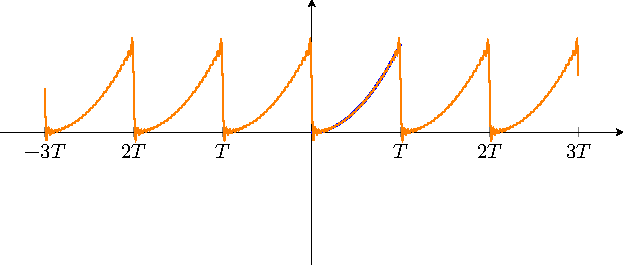
\includegraphics[width = 0.8\linewidth]{figures/half_range_expansion_Fourier.pdf}
    \caption{Fourier series expansion of \(f\left( t \right)\) on the interval \(\interval{0}{T}\), with the period \(T\).} % \label{}
\end{figure}
\begin{figure}[H]
    \centering
    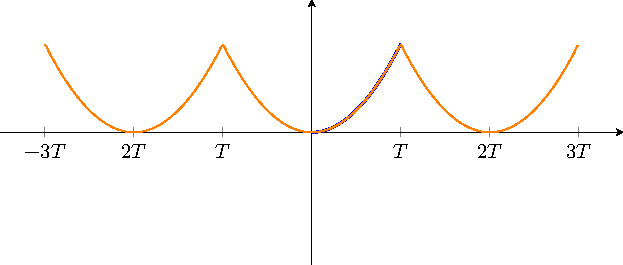
\includegraphics[width = 0.8\linewidth]{figures/half_range_expansion_Cosine.pdf}
    \caption{Fourier cosine series expansion of \(f\left( t \right)\) onto the interval \(\interval{-T}{T}\), with the period \(2T\).} % \label{}
\end{figure}
\begin{figure}[H]
    \centering
    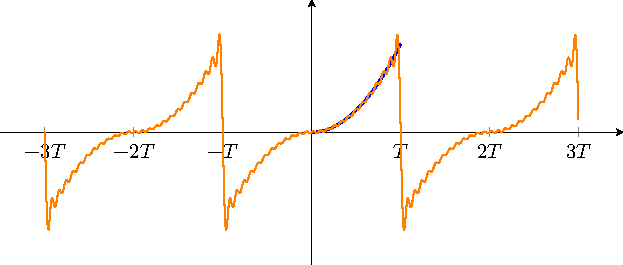
\includegraphics[width = 0.8\linewidth]{figures/half_range_expansion_Sine.pdf}
    \caption{Fourier sine series expansion of \(f\left( t \right)\) onto the interval \(\interval{-T}{T}\), with the period \(2T\).} % \label{}
\end{figure}
\part{Vector Calculus}
\section{Scalar Fields}
A scalar field is any function \(f : \mathbb{R}^n \to \mathbb{R}\),
that assigns a scalar value to every vector in \(\mathbb{R}^n\).
\subsection{Partial Derivatives}
The partial derivatives of a scalar field are defined as the derivative
of the function with respect to each variable:
\begin{equation*}
    \pdv{f}{x_i} \equiv f_{x_i} = \lim_{h \to 0} \frac{f\left( x_1, \: \ldots, \: x_i + h, \: \ldots, \: x_n \right) - f\left( x_1, \: \ldots, \: x_i, \: \ldots, \: x_n \right)}{h}
\end{equation*}
that is, the rate of change of the function in the \(x_i\) direction,
holding all other variables constant.
\subsection{Directional Derivatives}
To find the rate of change of a scalar field \(f\left( x_1, \: \ldots,
\: x_n \right)\) in the direction of a unit vector \(\mathbf{u} =
\left[ u_1, \: \ldots, \: u_n \right]\), we can scale the standard
basis vectors by the components of \(\mathbf{u}\):
\begin{equation*}
    D_{\mathbf{u}} f \equiv \pdv{f}{\symbf{u}} = \sum_{i=1}^{n} \pdv{f}{x_i} \frac{u_i}{\norm*{\symbf{u}}}.
\end{equation*}
This is known as the \textbf{directional derivative} of \(f\) in the direction of \(\mathbf{u}\).
\subsection{Gradient}
The gradient of a scalar field is an operator \(\grad : f \to
\mathbb{R}^n\) which maps a scalar field \(f\) to a vector field:
\begin{equation*}
    \grad{f} \equiv \symbf{\nabla} f = \left[ \pdv{}{x_1}, \: \ldots, \: \pdv{}{x_n} \right].
\end{equation*}
We can equivalently write the directional derivative as the dot product
of the gradient of \(f\) with the unit vector \(\mathbf{u}\):
\begin{equation*}
    D_{\mathbf{u}} f = \symbf{\nabla} f \cdot \hat{\mathbf{u}}.
\end{equation*}
\subsection{Gradient of a Scalar Field}
The gradient of a scalar field \(f\) is a vector field that points in
the direction of the greatest rate of change of \(f\), with magnitude
equal to the rate of change. That is:
\begin{itemize}
    \item \(\symbf{\nabla} f\) points in the direction of greatest increase of \(f\).
    \item \(-\symbf{\nabla} f\) points in the direction of greatest decrease of \(f\).
    \item \(\norm*{\symbf{\nabla} f}\) is the rate of increase of \(f\) in that direction.
\end{itemize}
\section{Vector Fields}
A vector field is any function \(\symbf{F} : \mathbb{R}^n \to
\mathbb{R}^n\), that assigns a vector to every vector in
\(\mathbb{R}^n\).
\subsection{Partial Derivatives}
The partial derivatives of a vector field are defined as the partial
derivatives of each component of the vector field:
\begin{equation*}
    \pdv{\symbf{F}}{x_i} = \symbf{F}_{x_i} = \left[ \pdv{F_1}{x_i}, \: \ldots, \: \pdv{F_n}{x_i} \right]
\end{equation*}
\subsection{Divergence}
The divergence of a vector field is an operator \(\divergence :
\symbf{F} \to \mathbb{R}\), which maps a vector field \(\symbf{F}\) to
a scalar:
\begin{equation*}
    \divergence \symbf{F} = \symbf{\nabla} \cdot \symbf{F} = \sum_{i=1}^{n} \pdv{F_i}{x_i}.
\end{equation*}
The divergence of a vector field measures the rate at which the vector
field flows out of a point \(P\).
\begin{itemize}
    \item When \(\divergence \symbf{F} > 0\), the vector field tends to
          flow away from \(P\) (source).
    \item When \(\divergence \symbf{F} < 0\), the vector field tends to
          flows towards \(P\) (sink).
    \item When \(\divergence \symbf{F} = 0\), the net flow of the
          vector field at \(P\) is zero (conservative).
\end{itemize}
\subsection{Curl}
The curl of a vector field is an operator \(\curl : \symbf{F} \to
\symbf{G}\), which maps a vector field \(\symbf{F} : \mathbb{R}^3 \to
\mathbb{R}^3\) to another vector field \(\symbf{G} : \mathbb{R}^3 \to
\mathbb{R}^3\):
\begin{equation*}
    \curl \symbf{F} = \symbf{\nabla} \times \symbf{F} =
    \begin{vmatrix}
        \symbf{i}              & \symbf{j}              & \symbf{k}              \\
        \displaystyle\pdv{}{x} & \displaystyle\pdv{}{y} & \displaystyle\pdv{}{z} \\
        F_1                    & F_2                    & F_3
    \end{vmatrix}
    .
\end{equation*}
The curl may also be defined for vector fields in \(\mathbb{R}^2\), where
\(F_3 = 0\). The curl of a vector field measures the rotation of the
vector field at a point \(P\).
\begin{itemize}
    \item When \(\curl \symbf{F} > 0\), the vector field tends to
          rotate counterclockwise around \(P\).
    \item When \(\curl \symbf{F} < 0\), the vector field tends to
          rotate clockwise around \(P\).
    \item When \(\curl \symbf{F} = 0\), the net rotation of the vector
          field around \(P\) is zero.
\end{itemize}
\section{Multiple Integrals}
Scalar functions can be integrated over regions in \(\mathbb{R}^n\)
through multiple integrals.
\subsection{Double Integrals}
When integrating over some region \(R\) in \(\mathbb{R}^2\), consider
the small subregion \(R_{ij}\) with area \(\Delta A_i = \Delta x_i
\Delta y_i\), so that the double integral of a function \(f\left( x, \:
y \right)\) over \(R\) is defined as the contribution of each
subregion:
\begin{equation*}
    \iint_{R} f\left( x, \: y \right) \odif{A} = \lim_{N \to \infty} \sum_{i=1}^{N} f\left( x_i, \: y_i \right) \Delta A_i.
\end{equation*}
To compute this integral, we must bound the region by two functions
\(g\) and \(h\) in either the \(x\)- or \(y\)-direction.
\begin{itemize}
    \item In the \(y\)-direction, the region is bounded by the curves:
          \begin{alignat*}{2}
              g\left( x \right) & \hspace{0.5em} \leqslant \hspace{0.5em} y &  & \hspace{0.5em} \leqslant \hspace{0.5em} h\left( x \right) \\
              a                 & \hspace{0.5em} \leqslant \hspace{0.5em} x &  & \hspace{0.5em} \leqslant \hspace{0.5em} b
          \end{alignat*}
          for some functions \(g\left( x \right)\) and \(h\left( x \right)\)
          so that
          \begin{equation*}
              \iint_{R} f\left( x, \: y \right) \odif{A} = \int_a^b \left[ \int_{g\left( x \right)}^{h\left( x \right)} f\left( x, \: y \right) \odif{y} \right] \odif{x}.
          \end{equation*}
          Here we are adding up vertical strips of width \(\odif{x}\),
          where each strips height is given by the distance between
          \(g\left( x \right)\) and \(h\left( x \right)\), weighted by
          the function \(f\left( x, \: y \right)\).
    \item In the \(x\)-direction, the region is bounded by the curves:
          \begin{alignat*}{2}
              c                 & \hspace{0.5em} \leqslant \hspace{0.5em} x &  & \hspace{0.5em} \leqslant \hspace{0.5em} d                 \\
              g\left( y \right) & \hspace{0.5em} \leqslant \hspace{0.5em} x &  & \hspace{0.5em} \leqslant \hspace{0.5em} h\left( y \right)
          \end{alignat*}
          for some functions \(g\left( y \right)\) and \(h\left( y \right)\)
          so that
          \begin{equation*}
              \iint_{R} f\left( x, \: y \right) \odif{A} = \int_c^d \left[ \int_{g\left( y \right)}^{h\left( y \right)} f\left( x, \: y \right) \odif{x} \right] \odif{y}.
          \end{equation*}
          Here we are adding up horizontal strips of width \(\odif{y}\),
          where each strips height is given by the distance between
          \(g\left( y \right)\) and \(h\left( y \right)\), weighted by
          the function \(f\left( x, \: y \right)\).
\end{itemize}
\subsection{Order of Integration}
By Fubini's theorem, any permutation of the order of integration of an
iterated integral is equivalent if the function being integrated is
integrable, that is if:
\begin{equation*}
    \int_R \abs*{f\left( \symbf{x} \right)} \odif{\symbf{x}} < \infty.
\end{equation*}
When applying Fubini's theorem, we must appropriately modify the bounds
of integration to account for the region \(R\). For example, if the region
is bounded by the curves:
\begin{equation*}
    R = \left\{ \left( x, \: y \right) : a \leqslant x \leqslant b, \: g\left( x \right) \leqslant y \leqslant h\left( x \right) \right\},
\end{equation*}
where \(g\) and \(h\) are invertible on the interval \(\interval{a}{b}\),
and the integral of a function \(f\left( x, \: y \right)\) over \(R\)
is given by:
\begin{equation*}
    \iint_R f\left( x, \: y \right) \odif{A} = \int_a^b \left[ \int_{g\left( x \right)}^{h\left( x \right)} f\left( x, \: y \right) \odif{y} \right] \odif{x},
\end{equation*}
we can equivalently integrate over the region \(R\) by reversing the
order of integration:
\begin{equation*}
    \iint_R f\left( x, \: y \right) \odif{A} = \int_{g\left( a \right)}^{h\left( b \right)} \left[ \int_{h^{-1}\left( y \right)}^{g^{-1}\left( y \right)} f\left( x, \: y \right) \odif{x} \right] \odif{y}.
\end{equation*}
Similarly, if the region is bounded by the curves:
\begin{equation*}
    R = \left\{ \left( x, \: y \right) : c \leqslant y \leqslant d, \: g\left( y \right) \leqslant x \leqslant h\left( y \right) \right\},
\end{equation*}
we can integrate over the region \(R\) by reversing the order of
integration:
\begin{equation*}
    \iint_R f\left( x, \: y \right) \odif{A} = \int_{g\left( c \right)}^{h\left( d \right)} \left[ \int_{h^{-1}\left( x \right)}^{g^{-1}\left( x \right)} f\left( x, \: y \right) \odif{y} \right] \odif{x}.
\end{equation*}
\subsection{Triple Integrals}
When integrating over some volume \(V\) in \(\mathbb{R}^3\), consider
the small subregion \(V_{ijk}\) with volume \(\Delta V_i = \Delta x_i
\Delta y_i \Delta z_i\), so that the triple integral of a function
\(f\left( x, \: y, \: z \right)\) over \(V\) is defined as the
contribution of each subregion:
\begin{equation*}
    \iiint_{V} f\left( x, \: y, \: z \right) \odif{V} = \lim_{N \to \infty} \sum_{i=1}^{N} f\left( x_i, \: y_i, \: z_i \right) \Delta V_i.
\end{equation*}
To compute this integral, we require three intervals for each variable
\(x\), \(y\), and \(z\), that enclose the volume \(V\). As we introduce
another dimension, the function bounding the innermost integral may
depend on both the outer variables. This integral may take the form:
\begin{equation*}
    \iiint_{V} f\left( x, \: y, \: z \right) \odif{V} = \int_a^b \left[ \int_c^d \left[ \int_g^h f\left( x, \: y, \: z \right) \odif{z} \right] \odif{y} \right] \odif{x}
\end{equation*}
for the volume enclosed by:
\begin{equation*}
    V = \left\{ \left( x, \: y, \: z \right) : a \leqslant x \leqslant b, \: c\left( x \right) \leqslant y \leqslant d\left( x \right), \: g\left( x, \: y \right) \leqslant z \leqslant h\left( x, \: y \right) \right\}.
\end{equation*}
Note that the bounds of any integral must not include any variables that
appear inside that integral. When modifying the order of integration,
we must ensure the same region is enclosed by the new bounds.
\subsection{Transformation of Coordinates}
In single variable calculus, we used a change of variables to simplify
integration by considering a transformation \(u = S\left( x \right)\),
to rewrite an integral in terms of \(u\), with the differential:
\begin{equation*}
    \odif{x} = \frac{1}{\odv{S\left( x \right)}{x}} \odif{u} = \odv{S^{-1}\left( u \right)}{u} \odif{u}
\end{equation*}
where \(x = S^{-1}\left( u \right)\) is the inverse transformation. This
concept can be extended to integrals with multiple variables by
considering the inverse transformation
\(x = T\left( u \right) = S^{-1}\left( u \right)\), where we can use
the chain rule to find the differential:
\begin{equation*}
    \odif{x} = \odv{T\left( u \right)}{u} \odif{u}.
\end{equation*}
To transform the coordinates in a multivariable integral, we must consider
a matrix of all the partial derivatives of a transformation. For the
transformation \(\symbf{x} = \symbf{T}\left( \symbf{u} \right)\),
consider the Jacobian matrix of partial derivatives:
\begin{equation*}
    \symbf{J} =
    \begin{bmatrix}
        \displaystyle\pdv{x_1}{u_1} & \cdots & \displaystyle\pdv{x_1}{u_n} \\
        \vdots                      & \ddots & \vdots                      \\
        \displaystyle\pdv{x_n}{u_1} & \cdots & \displaystyle\pdv{x_n}{u_n}
    \end{bmatrix}
    .
\end{equation*}
The determinant of this matrix is known as the Jacobian of a transformation,
and it gives us the factor by which the volume of the region is scaled
under the transformation, giving us the new differential:
\begin{equation*}
    \odif{\symbf{x}} = \abs*{\det{\symbf{J}}} \odif{\symbf{u}}.
\end{equation*}
Therefore, given a bijective transformation \(T : \Omega \subset \R^n \to \Omega'\subset \R^n\),
where \(T\) has continuous partial derivatives, an integral in
\(\symbf{x}\) can be transformed to an integral in \(\symbf{u}\) by:
\begin{equation*}
    \int_\Omega f\left( \symbf{x} \right) \odif{\symbf{x}} = \int_{\Omega'} f\left( \symbf{T}\left( \symbf{u} \right) \right) \abs*{\det{\symbf{J}}} \odif{\symbf{u}}.
\end{equation*}
\subsubsection{Polar Coordinates (2D)}
To transform a Cartesian coordinate system to polar coordinates,
consider the transformation:
\begin{align*}
    x & = r \cos{\theta} & r      & = \sqrt{x^2 + y^2}                    \\
    y & = r \sin{\theta} & \theta & = \arctan{\left( \frac{y}{x} \right)}
\end{align*}
for \(r \geqslant 0\) and \(0 \leqslant \theta \leqslant 2\pi\). This transformation has
the Jacobian matrix:
\begin{equation*}
    \symbf{J} =
    \begin{bmatrix}
        \displaystyle\pdv{x}{r} & \displaystyle\pdv{x}{\theta} \\
        \displaystyle\pdv{y}{r} & \displaystyle\pdv{y}{\theta}
    \end{bmatrix}
    =
    \begin{bmatrix}
        \cos{\theta} & -r \sin{\theta} \\
        \sin{\theta} & r \cos{\theta}
    \end{bmatrix}
\end{equation*}
with the determinant:
\begin{equation*}
    \abs*{\det{\symbf{J}}} = r \cos^2{\theta} + r \sin^2{\theta} = r.
\end{equation*}
Therefore, the differential in polar coordinates is:
\begin{equation*}
    \odif{x} \odif{y} = r \odif{r} \odif{\theta},
\end{equation*}
giving the integral transformation:
\begin{equation*}
    \iint_{R} f\left( x, \: y \right) \odif{x} \odif{y} = \iint_{R'} f\left( r, \: \theta \right) r \odif{r} \odif{\theta}.
\end{equation*}
The gradient of this transformation can be computed by applying the
chain rule:
\begin{align*}
    \pdv{}{x} & = \pdv{r}{x} \pdv{}{r} + \pdv{\theta}{x} \pdv{}{\theta} \\
    \pdv{}{y} & = \pdv{r}{y} \pdv{}{r} + \pdv{\theta}{y} \pdv{}{\theta}
\end{align*}
The partial derivatives in these expressions are given by:
\begin{align*}
    \pdv{r}{x} & = \frac{x}{r} = \cos{\theta} & \pdv{\theta}{x} & = -\frac{y}{r^2} = -\frac{1}{r}\sin{\theta} \\
    \pdv{r}{y} & = \frac{y}{r} = \sin{\theta} & \pdv{\theta}{y} & = \frac{x}{r^2} = \frac{1}{r}\cos{\theta}
\end{align*}
so that the gradient in polar coordinates is defined:
\begin{align*}
    \symbf{\nabla} & = \symbf{e}_x \pdv{}{x} + \symbf{e}_y \pdv{}{y}                                                                                                                                             \\
                   & = \symbf{e}_x \left[ \cos{\theta} \pdv{}{r} - \frac{1}{r} \sin{\theta} \pdv{}{\theta} \right] + \symbf{e}_y \left[ \sin{\theta} \pdv{}{r} + \frac{1}{r} \cos{\theta} \pdv{}{\theta} \right] \\
                   & = \left[ \cos{\theta} \symbf{e}_x + \sin{\theta} \symbf{e}_y \right] \pdv{}{r} + \left[ \cos{\theta} \symbf{e}_y - \sin{\theta} \symbf{e}_x \right] \frac{1}{r} \pdv{}{\theta}              \\
                   & = \symbf{e}_r \pdv{}{r} + \symbf{e}_\theta \frac{1}{r} \pdv{}{\theta}
\end{align*}
giving the transformed basis vectors:
\begin{align*}
    \symbf{e}_r      & = \cos{\theta} \symbf{e}_x + \sin{\theta} \symbf{e}_y \\
    \symbf{e}_\theta & = \cos{\theta} \symbf{e}_y - \sin{\theta} \symbf{e}_x
\end{align*}
\subsubsection{Cylindrical Coordinates (3D)}
To transform a Cartesian coordinate system to cylindrical coordinates,
consider the transformation:
\begin{align*}
    x & = r \cos{\theta} & r      & = \sqrt{x^2 + y^2}                    \\
    y & = r \sin{\theta} & \theta & = \arctan{\left( \frac{y}{x} \right)} \\
    z & = z              & z      & = z
\end{align*}
for \(r \geqslant 0\), \(0 \leqslant \theta \leqslant 2\pi\), and \(-\infty < z < \infty\).
This transformation has the Jacobian matrix:
\begin{equation*}
    \symbf{J} =
    \begin{bmatrix}
        \displaystyle\pdv{x}{r} & \displaystyle\pdv{x}{\theta} & \displaystyle\pdv{x}{z} \\
        \displaystyle\pdv{y}{r} & \displaystyle\pdv{y}{\theta} & \displaystyle\pdv{y}{z} \\
        \displaystyle\pdv{z}{r} & \displaystyle\pdv{z}{\theta} & \displaystyle\pdv{z}{z}
    \end{bmatrix}
    =
    \begin{bmatrix}
        \cos{\theta} & -r \sin{\theta} & 0 \\
        \sin{\theta} & r \cos{\theta}  & 0 \\
        0            & 0               & 1
    \end{bmatrix}
\end{equation*}
with the determinant:
\begin{equation*}
    \abs*{\det{\symbf{J}}} = r \cos^2{\theta} + r \sin^2{\theta} = r.
\end{equation*}
Therefore, the differential in cylindrical coordinates is:
\begin{equation*}
    \odif{x} \odif{y} \odif{z} = r \odif{r} \odif{\theta} \odif{z},
\end{equation*}
giving the integral transformation:
\begin{equation*}
    \iiint_{V} f\left( x, \: y, \: z \right) \odif{x} \odif{y} \odif{z} = \iiint_{V'} f\left( r, \: \theta, \: z \right) r \odif{r} \odif{\theta} \odif{z}.
\end{equation*}
The gradient of this transformation can be computed by applying the
chain rule:
\begin{align*}
    \pdv{}{x} & = \pdv{r}{x} \pdv{}{r} + \pdv{\theta}{x} \pdv{}{\theta} + \pdv{z}{x} \pdv{}{z} \\
    \pdv{}{y} & = \pdv{r}{y} \pdv{}{r} + \pdv{\theta}{y} \pdv{}{\theta} + \pdv{z}{y} \pdv{}{z} \\
    \pdv{}{z} & = \pdv{r}{z} \pdv{}{r} + \pdv{\theta}{z} \pdv{}{\theta} + \pdv{z}{z} \pdv{}{z}
\end{align*}
The partial derivatives in these expressions are given by:
\begin{align*}
    \pdv{r}{x} & = \frac{x}{r} = \cos{\theta} & \pdv{\theta}{x} & = -\frac{y}{r^2} = -\frac{1}{r}\sin{\theta} & \pdv{z}{x} & = 0 \\
    \pdv{r}{y} & = \frac{y}{r} = \sin{\theta} & \pdv{\theta}{y} & = \frac{x}{r^2} = \frac{1}{r}\cos{\theta}   & \pdv{z}{y} & = 0 \\
    \pdv{r}{z} & = 0                          & \pdv{\theta}{z} & = 0                                         & \pdv{z}{z} & = 1
\end{align*}
so that the gradient in cylindrical coordinates is defined:
\begin{align*}
    \symbf{\nabla} & = \symbf{e}_x \pdv{}{x} + \symbf{e}_y \pdv{}{y} + \symbf{e}_z \pdv{}{z}                                                                                                                                             \\
                   & = \symbf{e}_x \left[ \cos{\theta} \pdv{}{r} - \frac{1}{r} \sin{\theta} \pdv{}{\theta} \right] + \symbf{e}_y \left[ \sin{\theta} \pdv{}{r} + \frac{1}{r} \cos{\theta} \pdv{}{\theta} \right] + \symbf{e}_z \pdv{}{z} \\
                   & = \left[ \cos{\theta} \symbf{e}_x + \sin{\theta} \symbf{e}_y \right] \pdv{}{r} + \left[ \cos{\theta} \symbf{e}_y - \sin{\theta} \symbf{e}_x \right] \frac{1}{r} \pdv{}{\theta} + \symbf{e}_z \pdv{}{z}              \\
                   & = \symbf{e}_r \pdv{}{r} + \symbf{e}_\theta \frac{1}{r} \pdv{}{\theta} + \symbf{e}_z \pdv{}{z}
\end{align*}
giving the transformed basis vectors:
\begin{align*}
    \symbf{e}_r      & = \cos{\theta} \symbf{e}_x + \sin{\theta} \symbf{e}_y \\
    \symbf{e}_\theta & = \cos{\theta} \symbf{e}_y - \sin{\theta} \symbf{e}_x \\
    \symbf{e}_z      & = \symbf{e}_z
\end{align*}
\subsubsection{Spherical Coordinates (3D)}
To transform a Cartesian coordinate system to spherical coordinates,
consider the transformation:
\begin{align*}
    x & = r \cos{\theta} \sin{\phi} & r      & = \sqrt{x^2 + y^2 + z^2}              \\
    y & = r \sin{\theta} \sin{\phi} & \theta & = \arctan{\left( \frac{y}{x} \right)} \\
    z & = r \cos{\phi}              & \phi   & = \arccos{\left( \frac{z}{r} \right)}
\end{align*}
for \(r \geqslant 0\), \(0 \leqslant \theta \leqslant 2\pi\), and \(0 \leqslant \phi \leqslant \pi\).
This transformation has the Jacobian matrix:
\begin{equation*}
    \symbf{J} =
    \begin{bmatrix}
        \displaystyle\pdv{x}{r} & \displaystyle\pdv{x}{\phi} & \displaystyle\pdv{x}{\theta} \\
        \displaystyle\pdv{y}{r} & \displaystyle\pdv{y}{\phi} & \displaystyle\pdv{y}{\theta} \\
        \displaystyle\pdv{z}{r} & \displaystyle\pdv{z}{\phi} & \displaystyle\pdv{z}{\theta}
    \end{bmatrix}
    =
    \begin{bmatrix}
        \cos{\theta} \sin{\phi} & r \cos{\theta} \cos{\phi} & -r \sin{\theta} \sin{\phi} \\
        \sin{\theta} \sin{\phi} & r \sin{\theta} \cos{\phi} & r \cos{\theta} \sin{\phi}  \\
        \cos{\phi}              & -r \sin{\phi}             & 0
    \end{bmatrix}
\end{equation*}
with the determinant:
\begin{equation*}
    \abs*{\det{\symbf{J}}} = r^2 \sin{\phi}.
\end{equation*}
Therefore, the differential in spherical coordinates is:
\begin{equation*}
    \odif{x} \odif{y} \odif{z} = r^2 \sin{\phi} \odif{r} \odif{\phi} \odif{\theta},
\end{equation*}
giving the integral transformation:
\begin{equation*}
    \iiint_{V} f\left( x, \: y, \: z \right) \odif{x} \odif{y} \odif{z} = \iiint_{V'} f\left( r, \: \theta, \: \phi \right) r^2 \sin{\phi} \odif{r} \odif{\theta} \odif{\phi}.
\end{equation*}
The gradient of this transformation can be computed by applying the
chain rule:
\begin{align*}
    \pdv{}{x} & = \pdv{r}{x} \pdv{}{r} + \pdv{\phi}{x} \pdv{}{\phi} + \pdv{\theta}{x} \pdv{}{\theta} \\
    \pdv{}{y} & = \pdv{r}{y} \pdv{}{r} + \pdv{\phi}{y} \pdv{}{\phi} + \pdv{\theta}{y} \pdv{}{\theta} \\
    \pdv{}{z} & = \pdv{r}{z} \pdv{}{r} + \pdv{\phi}{z} \pdv{}{\phi} + \pdv{\theta}{z} \pdv{}{\theta}
\end{align*}
The partial derivatives in these expressions are given by:
\begin{align*}
    \pdv{r}{x} & = \frac{x}{r} = \cos{\theta} \sin{\phi} & \pdv{\phi}{x} & = -\frac{z\left( - x r^{-3} \right)}{\sqrt{1 - \frac{z^2}{r^2}}} = \frac{\cos{\theta}\cos{\phi}}{r} & \pdv{\theta}{x} & = -\frac{y}{x^2 + y^2} = -\frac{\sin{\theta}}{r \sin{\phi}} \\
    \pdv{r}{y} & = \frac{y}{r} = \sin{\theta} \sin{\phi} & \pdv{\phi}{y} & = -\frac{z\left( - y r^{-3} \right)}{\sqrt{1 - \frac{z^2}{r^2}}} = \frac{\sin{\theta}\cos{\phi}}{r} & \pdv{\theta}{y} & = \frac{x}{x^2 + y^2} = \frac{\cos{\theta}}{r \sin{\phi}}   \\
    \pdv{r}{z} & = \frac{z}{r} = \cos{\phi}              & \pdv{\phi}{z} & = -\frac{\left( r - z^2r^{-1} \right)r^{-2}}{\sqrt{1 - \frac{z^2}{r^2}}} = -\frac{\sin{\phi}}{r}    & \pdv{\theta}{z} & = 0
\end{align*}
so that the gradient in spherical coordinates is defined:
\begin{align*}
    \symbf{\nabla} & = \symbf{e}_x \pdv{}{x} + \symbf{e}_y \pdv{}{y} + \symbf{e}_z \pdv{}{z}                                                    \\
                   & =
    \begin{aligned}[t]
          & \symbf{e}_x \left[ \cos{\theta} \sin{\phi} \pdv{}{r} + \frac{\cos{\theta}\cos{\phi}}{r} \pdv{}{\phi} - \frac{\sin{\theta}}{r \sin{\phi}} \pdv{}{\theta} \right] \\
        + & \symbf{e}_y \left[ \sin{\theta} \sin{\phi} \pdv{}{r} + \frac{\sin{\theta}\cos{\phi}}{r} \pdv{}{\phi} + \frac{\cos{\theta}}{r \sin{\phi}} \pdv{}{\theta} \right] \\
        + & \symbf{e}_z \left[ \cos{\phi} \pdv{}{r} - \frac{\sin{\phi}}{r} \pdv{}{\phi} \right]
    \end{aligned}
    \\
                   & =
    \begin{aligned}[t]
          & \left[ \cos{\theta} \sin{\phi} \symbf{e}_x + \sin{\theta} \sin{\phi} \symbf{e}_y + \cos{\phi} \symbf{e}_z \right] \pdv{}{r}              \\
        + & \left[ \cos{\theta}\cos{\phi} \symbf{e}_x + \sin{\theta}\cos{\phi} \symbf{e}_y - \sin{\phi} \symbf{e}_z \right] \frac{1}{r} \pdv{}{\phi} \\
        + & \left[ \cos{\theta} \symbf{e}_y - \sin{\theta} \symbf{e}_x \right] \frac{1}{r \sin{\phi}} \pdv{}{\theta}
    \end{aligned}
    \\
                   & = \symbf{e}_r \pdv{}{r} + \symbf{e}_\phi \frac{1}{r} \pdv{}{\phi} + \symbf{e}_\theta \frac{1}{r \sin{\phi}} \pdv{}{\theta}
\end{align*}
giving the transformed basis vectors:
\begin{align*}
    \symbf{e}_r      & = \cos{\theta} \sin{\phi} \symbf{e}_x + \sin{\theta} \sin{\phi} \symbf{e}_y + \cos{\phi} \symbf{e}_z \\
    \symbf{e}_\phi   & = \cos{\theta}\cos{\phi} \symbf{e}_x + \sin{\theta}\cos{\phi} \symbf{e}_y - \sin{\phi} \symbf{e}_z   \\
    \symbf{e}_\theta & = \cos{\theta} \symbf{e}_y - \sin{\theta} \symbf{e}_x
\end{align*}
\subsection{Physical Interpretation of Integrals}
Integrals can be used to represent various physical quantities.
\subsubsection{Measures}
The measure of a region \(R \in \R^n\) is given by the integral of the
unit density function \(\rho\left( \symbf{x} \right) = 1\) over \(R\):
\begin{equation*}
    \mu = \int_R \odif{\symbf{x}}.
\end{equation*}
\begin{itemize}
    \item In 1D, the measure represents the length of \(R\).
    \item In 2D, the measure represents the area of \(R\).
    \item In 3D, the measure represents the volume of \(R\).
\end{itemize}
\subsubsection{Mass}
The mass of a region \(R \in \R^n\) is given by the integral of the
density function \(\rho\left( \symbf{x} \right)\) over \(R\):
\begin{equation*}
    M = \int_R \rho\left( \symbf{x} \right) \odif{\symbf{x}}.
\end{equation*}
\subsubsection{Centroid}
The centroid (average position) of a region \(R \in \R^n\) with uniform
density \(\rho\left( \symbf{x} \right) = 1\) is given by:
\begin{equation*}
    \symbf{c} = \frac{1}{\mu} \int_R \symbf{x} \odif{\symbf{x}}.
\end{equation*}
\subsubsection{Centre of Mass}
The centre of mass of a region \(R \in \R^n\) with density function
\(\rho\left( \symbf{x} \right)\) is given by:
\begin{equation*}
    \symbf{c}_{\rho} = \frac{1}{M} \int_R \rho\left( \symbf{x} \right) \symbf{x} \odif{\symbf{x}}.
\end{equation*}
\subsubsection{Average Value}
The average value of a function \(f\left( \symbf{x} \right)\) over a
region \(R \in \R^n\) is given by:
\begin{equation*}
    \bar{f} = \frac{1}{\mu} \int_R f\left( \symbf{x} \right) \odif{\symbf{x}}.
\end{equation*}
\section{Line Integrals}
\subsection{Parametric Curves}
A path is a continuous function \(\symbf{r}\left( t \right)\) that maps
a parameter \(t\) to a point in \(\R^n\):
\begin{equation*}
    \symbf{r}\left( t \right) =
    \begin{bmatrix}
        x_1\left( t \right) \\
        x_2\left( t \right) \\
        \vdots              \\
        x_n\left( t \right)
    \end{bmatrix}
    .
\end{equation*}
A curve \(\mathscr{C}\) in \(\R^n\) is the set of points corresponding
to the range of the path \(\symbf{r}\left( t \right)\), where
\(a \leqslant t \leqslant b\):
\begin{equation*}
    \mathscr{C} = \left\{ \symbf{r}\left( t \right) : a \leqslant t \leqslant b \right\}.
\end{equation*}
A path is closed if \(\symbf{r}\left( a \right) = \symbf{r}\left( b \right)\).
The velocity of a path is given by the derivative of the path:
\begin{equation*}
    \symbf{v}\left( t \right) = \symbf{r}'\left( t \right) =
    \begin{bmatrix}
        x_1'\left( t \right) \\
        x_2'\left( t \right) \\
        \vdots               \\
        x_n'\left( t \right)
    \end{bmatrix}
    .
\end{equation*}
This allows us to define the speed of the path as the magnitude of the
velocity:
\begin{equation*}
    \norm*{\symbf{v}\left( t \right)} = \norm*{\symbf{r}'\left( t \right)} = \sqrt{x_1'^2 + x_2'^2 + \cdots + x_n'^2}.
\end{equation*}
Integrals along paths are called line integrals.
\subsection{Line Integrals of Scalar Fields}
Line integrals of scalar fields have the form:
\begin{equation*}
    \int_{\mathscr{C}} f \odif{r}
\end{equation*}
These integrals represent a weighted sum over the scalar field \(f\)
along a curve parametrised by the path \(\symbf{r}\left( t \right)\).
To compute the differential element \(\odif{r}\), consider its
relationship with the canonical Euclidean differential elements:
\begin{equation*}
    \odif{r}^2 = \sum_{i = 1}^n \odif{x}_i^2 \implies \odif{r} = \sqrt{\sum_{i = 1}^n \odif{x}_i^2} = \sqrt{\sum_{i = 1}^n \left( \odv{x_i}{t} \right)^2} \odif{t} = \norm*{\symbf{r}'\left( t \right)} \odif{t}.
\end{equation*}
Using the chain rule, we can also represent the differential element
\(\odif{r}\) using the form:
\begin{equation*}
    \odif{r} = \odv{r}{t} \odif{t}
\end{equation*}
so that
\begin{equation*}
    \odv{r}{t} = \norm*{\symbf{r}'\left( t \right)}
\end{equation*}
represents the speed of the path. Therefore, the line integral of \(f\)
along the curve \(\mathscr{C}\) is given by:
\begin{equation*}
    \int_{\mathscr{C}} f \odif{r} = \int_a^b f\left( \symbf{r}\left( t \right) \right) \norm*{\symbf{r}'\left( t \right)} \odif{t}.
\end{equation*}
\subsubsection{Arc Length}
The arc length of the curve \(\mathscr{C}\) is a function which
measures the length of the path \(\symbf{r}\left( t \right)\) from
\(a\) to \(\tau\). It is defined as the line integral of a uniform
field:
\begin{equation*}
    s\left( \tau \right) = \int_a^\tau \odif{r} = \int_a^\tau \norm*{\symbf{r}'\left( t \right)} \odif{t}.
\end{equation*}
The total length of the curve \(\mathscr{C}\) is therefore:
\begin{equation*}
    L = s\left( b \right) = \int_{\mathscr{C}} \odif{r} = \int_a^b \norm*{\symbf{r}'\left( t \right)} \odif{t}.
\end{equation*}
\subsection{Line Integrals of Vector Fields}
Line integrals of vector fields have the form:
\begin{equation*}
    W = \int_{\mathscr{C}} \symbf{F} \cdot \odif{\symbf{r}}
\end{equation*}
These integrals represent the work done by the vector field \(\symbf{F}\)
along a curve parametrised by the path \(\symbf{r}\left( t \right)\).
The differential element \(\odif{\symbf{r}}\) can be computed using the
chain rule:
\begin{equation*}
    \odif{\symbf{r}} = \odv{\symbf{r}}{t} \odif{t} = \symbf{r}'\left( t \right) \odif{t}
\end{equation*}
where \(\symbf{r}'\left( t \right)\) is the velocity of the path.
Therefore, the line integral of \(\symbf{F}\) along the curve
\(\mathscr{C}\) is given by:
\begin{equation*}
    \int_{\mathscr{C}} \symbf{F} \cdot \odif{\symbf{r}} = \int_a^b \symbf{F}\left( \symbf{r}\left( t \right) \right) \cdot \symbf{r}'\left( t \right) \odif{t}.
\end{equation*}
\subsubsection{Circulation}
When the path \(\symbf{r}\left( t \right)\) is closed, line integrals
of vector fields along \(\mathscr{C}\) can be denoted as:
\begin{equation*}
    \Gamma = \oint_{\mathscr{C}} \symbf{F} \cdot \odif{\symbf{r}}
\end{equation*}
where \(\Gamma\) is the circulation of the vector field \(\symbf{F}\)
along \(\mathscr{C}\).
\subsubsection{Conservative Fields}
The vector field \(\symbf{F}\) is called conservative when
\begin{equation*}
    \symbf{F} = \symbf{\nabla} \phi
\end{equation*}
for some scalar function \(\phi\). When \(\symbf{F}\) is conservative,
the line integral along \(\mathscr{C}\) is path independent:
\begin{equation*}
    \int_{\mathscr{C}} \symbf{F} \cdot \odif{\symbf{r}} = \int_{\mathscr{C}} \symbf{\nabla}\phi \cdot \odif{\symbf{r}} = \int_a^b \symbf{\nabla}\phi\left( \symbf{r}\left( t \right) \right) \cdot \symbf{r}'\left( t \right) \odif{t} = \int_a^b \odv{\phi\left( \symbf{r}\left( t \right) \right)}{t} \odif{t} = \phi\left( \symbf{r}\left( b \right) \right) - \phi\left( \symbf{r}\left( a \right) \right).
\end{equation*}
When \(\symbf{r}\left( t \right)\) is a closed path,
the circulation is zero:
\begin{equation*}
    \Gamma = \oint_{\mathscr{C}} \symbf{F} \cdot \odif{\symbf{r}} = \phi\left( \symbf{r}\left( b \right) \right) - \phi\left( \symbf{r}\left( a \right) \right) = 0.
\end{equation*}
\section{Surface Integrals}
\subsection{Parametric Surfaces}
Consider the parametric function \(\symbf{r}\left( s,\: t \right)\)
that maps the parameters \(s\) and \(t\) to a point in \(\R^3\):
\begin{equation*}
    \symbf{r}\left( s,\: t \right) =
    \begin{bmatrix}
        x\left( s,\: t \right) \\
        y\left( s,\: t \right) \\
        z\left( s,\: t \right)
    \end{bmatrix}
\end{equation*}
A surface \(\mathscr{S}\) in \(\R^3\) is the set of points corresponding
to the range of the parametric function \(\symbf{r}\left( s,\: t \right)\),
where \(a \leqslant s \leqslant b\) and \(c \leqslant t \leqslant d\):
\begin{equation*}
    \mathscr{S} = \left\{ \symbf{r}\left( s,\: t \right) : a \leqslant s \leqslant b, \: c \leqslant t \leqslant d \right\}.
\end{equation*}
When the partial derivatives of \(\symbf{r}\) are linearly independent,
we can define the normal vector to the surface:
\begin{equation*}
    \symbf{n} = \symbf{r}_s \times \symbf{r}_t.
\end{equation*}
Integrals over surfaces are called surface integrals.
\subsection{Surface Integrals of Scalar Fields}
Surface integrals of scalar fields have the form:
\begin{equation*}
    \iint_{\mathscr{S}} f \odif{\sigma}
\end{equation*}
These integrals represent the weighted area over the scalar field \(f\)
over the surface parametrised by \(\symbf{r}\left( s,\: t \right)\).
The differential element \(\odif{\sigma}\) is given by
\begin{equation*}
    \odif{\sigma} = \norm*{\symbf{r}_s \times \symbf{r}_t} \odif{s} \odif{t}
\end{equation*}
where \(\norm*{\symbf{r}_s \times \symbf{r}_t}\) represents the area of
the parallelogram spanned by \(\symbf{r}_s\) and \(\symbf{r}_t\).
Therefore, the surface integral of \(f\) over the surface \(\mathscr{S}\)
is given by:
\begin{equation*}
    \iint_{\mathscr{S}} f \odif{\sigma} = \int_c^d \int_a^b f\left( \symbf{r}\left( s,\: t \right) \right) \norm*{\symbf{r}_s \times \symbf{r}_t} \odif{s} \odif{t}.
\end{equation*}
\subsubsection{Surface Area}
The surface area of the surface \(\mathscr{S}\) is defined as the
surface integral of a uniform field:
\begin{equation*}
    A = \iint_{\mathscr{S}} \odif{\sigma} = \int_c^d \int_a^b \norm*{\symbf{r}_s \times \symbf{r}_t} \odif{s} \odif{t}.
\end{equation*}
\subsection{Surface Integrals of Vector Fields}
Surface integrals of vector fields have the form:
\begin{equation*}
    \Phi = \iint_{\mathscr{S}} \symbf{F} \cdot \odif{\symbf{\sigma}}
\end{equation*}
These integrals represent the flux of the vector field \(\symbf{F}\)
through the surface parametrised by \(\symbf{r}\left( s,\: t \right)\).
The differential element \(\odif{\symbf{\sigma}}\) is given by
\begin{equation*}
    \odif{\symbf{\sigma}} = \hat{\symbf{n}} \odif{\sigma} = \left( \symbf{r}_s \times \symbf{r}_t \right) \odif{s} \odif{t}
\end{equation*}
where \(\symbf{r}_s \times \symbf{r}_t\) represents the normal vector to
the surface \(\mathscr{S}\).
Therefore, the surface integral of \(\symbf{F}\) over the surface
\(\mathscr{S}\) is given by:
\begin{equation*}
    \Phi = \iint_{\mathscr{S}} \symbf{F} \cdot \odif{\symbf{\sigma}} = \iint_{\mathscr{S}} \left( \symbf{F} \cdot \hat{\symbf{n}} \right) \odif{\sigma} = \int_c^d \int_a^b \symbf{F}\left( \symbf{r}\left( s,\: t \right) \right) \cdot \left( \symbf{r}_s \times \symbf{r}_t \right) \odif{s} \odif{t}.
\end{equation*}
Note that this integral represents the outward or inward flow of
\(\symbf{F}\) through \(\mathscr{S}\), where the direction of flow
depends on the sign of \(\symbf{n}\).
\section{Fundamental Theorems of Calculus}
The three vector calculus operators have corresponding theorems which
generalise the Fundamental Theorem of Calculus to higher dimensions.
These results are commonly used to simplify line and surface integrals.
\subsection{Fundamental Theorem of Calculus Part II}
Consider the continuously differentiable function \(F:\interval{a}{b}
\to \R\), then
\begin{equation*}
    \int_a^b \odv{F}{x} \odif{x} = F\left( b \right) - F\left( a \right).
\end{equation*}
This theorem states that the integral of the derivative of \(F\) is
equal to the difference of the values of the function at the endpoints.
\subsection{Fundamental Theorem of Line Integrals (Gradient Theorem)}
Consider the differentiable scalar function \(\phi:\R^n \to \R\). Let
\(\mathscr{C}\) be a curve parametrised by \(\symbf{r}\left( t
\right)\), where \(a \leq t \leq b\), then
\begin{equation*}
    \int_{\mathscr{C}} \symbf{\nabla} \phi \cdot \odif{\symbf{r}} = \phi\left( \symbf{r}\left( b \right) \right) - \phi\left( \symbf{r}\left( a \right) \right).
\end{equation*}
This theorem states that line integrals through conservative fields
\(\symbf{F} = \symbf{\nabla} \phi\) are path independent.
\subsection{Gauss's Theorem (Divergence Theorem)}
Consider the closed region \(R \in \R^n\) with boundary \(\partial R\)
and let \(\symbf{F}:R \to \R^n\) be a continuously differentiable
vector field in \(R\). Then,
\begin{equation*}
    \underbrace{\int \cdots \int_R}_n \left( \symbf{\nabla} \cdot \symbf{F} \right) \odif{\symbf{x}} = \underbrace{\oint \cdots \oint_{\partial R}}_{n-1} \symbf{F} \cdot \odif{\symbf{\sigma}}.
\end{equation*}
This theorem states that the volume integral of the divergence of a
vector field \(\symbf{F}\) over the region \(R\) is equal to the surface
integral of \(\symbf{F}\) over the boundary \(\partial R\).
\subsection{Stoke's Theorem (Curl Theorem)}
Consider the surface \(\mathscr{S}\) parametrised by \(\symbf{r}\left(
s,\: t \right)\), with boundary \(\partial \mathscr{S}\) oriented
positively with respect to the normal vector \(\symbf{n}\), and let
\(\symbf{F}:\R^3 \to \R^3\) be a continuously differentiable vector
field in \(\mathscr{S}\). Then,
\begin{equation*}
    \iint_{\mathscr{S}} \left( \symbf{\nabla} \times \symbf{F} \right) \cdot \odif{\symbf{\sigma}} = \oint_{\partial \mathscr{S}} \symbf{F} \cdot \odif{\symbf{r}}.
\end{equation*}
This theorem states that the surface integral of the curl of a vector
field over the surface \(\mathscr{S}\) is equal to the line integral of
\(\symbf{F}\) along the boundary \(\partial \mathscr{S}\).
\subsection{Green's Theorem}
Consider the bounded region \(R \in \R^2\) with boundary \(\partial R\)
oriented positively (traversed in the counterclockwise direction) and
let \(\symbf{F}:R \to \R^2\) be a continuously differentiable vector
field in \(\R\). Then,
\begin{equation*}
    \iint_R \left( \symbf{\nabla} \times \symbf{F} \right) \odif{A} = \oint_{\partial R} \symbf{F} \cdot \odif{\symbf{r}}.
\end{equation*}
This expands to
\begin{equation*}
    \iint_R \left( \pdv{\symbf{F}_2}{x} - \pdv{\symbf{F}_1}{y} \right) \odif{x} \odif{y} = \oint_{\partial R} \symbf{F}_1 \odif{x} + \symbf{F}_2 \odif{y}.
\end{equation*}
This theorem states that the area integral of the curl of a vector field
\(\symbf{F}\) is equal to the line integral of \(\symbf{F}\) along the
boundary \(\partial R\). Green's theorem is a special case of both the
divergence and curl theorems in 2 dimensions.
\part{Ordinary Differential Equations}
\section{Laplace Transform}
Consider a forced linear constant-coefficient differential equation of
the form:
\begin{equation*}
    a_n y^{\left( n \right)}\left( t \right) + a_{n-1} y^{\left( n-1 \right)}\left( t \right) + \cdots + a_1 y'\left( t \right) + a_0 y\left( t \right) = f\left( t \right)
\end{equation*}
with initial conditions \(y\left( 0 \right) = y_0\), \(y'\left( 0 \right) = y_1\), \(\ldots\), \(y^{\left( n-1 \right)}\left( 0 \right) = y_{n-1}\).
Certain choices of \(f\left( t \right)\) can make the solution to this
differential equation difficult to determine using methods such as
undetermined coefficients or variation of parameters, due to the
complexity of the integrals involved. Here we introduce the Laplace
transform, which allows us to transform a differential equation into
an algebraic equation. The Laplace transform of a function
\(f\left( t \right)\) is defined as:
\begin{equation*}
    \mathscr{L}\left\{ f\left( t \right) \right\} \equiv F\left( s \right) = \int_0^\infty f\left( t \right) e^{-st} \odif{t},
\end{equation*}
where \(s\) is a complex number. Consider the Laplace transform of
\(\displaystyle \odv{y\left( t \right)}{t}\):
\begin{align*}
    \mathscr{L}\left\{ \odv{y\left( t \right)}{t} \right\} & = \int_0^\infty \odv{y\left( t \right)}{t} e^{-st} \odif{t}                                              \\
                                                           & = \left. e^{-st} y\left( t \right) \right|_0^\infty + s \int_0^\infty e^{-st} y\left( t \right) \odif{t} \\
                                                           & = s Y\left( s \right) - y\left( 0 \right).
\end{align*}
Now consider the Laplace transform of \(\displaystyle \odv[order=2]{y\left( t \right)}{t}\):
\begin{align*}
    \mathscr{L}\left\{ \odv[order=2]{y\left( t \right)}{t} \right\} & = \int_0^\infty \odv[order=2]{y\left( t \right)}{t} e^{-st} \odif{t}                                                                                              \\
                                                                    & = \left. e^{-st} y'\left( t \right) \right|_0^\infty + \left. s e^{-st} y\left( t \right) \right|_0^\infty + s^2 \int_0^\infty e^{-st} y\left( t \right) \odif{t} \\
                                                                    & = s^2 Y\left( s \right) - s y\left( 0 \right) - y'\left( 0 \right).
\end{align*}
Therefore, we can deduce that the Laplace transform of
\(\displaystyle \odv[order=n]{y\left( t \right)}{t}\) is given by:
\begin{align*}
    \mathscr{L}\left\{ \odv[order=n]{y\left( t \right)}{t} \right\} & = s^n Y\left( s \right) - \left[ s^{n-1} y\left( 0 \right) + s^{n-2} y'\left( 0 \right) + \cdots + y^{\left( n-1 \right)}\left( 0 \right) \right] \\
                                                                    & = s^n Y\left( s \right) - \sum_{k=0}^{n-1} s^{n-1-k} y^{\left( k \right)}\left( 0 \right).
\end{align*}
Using this property, we can transform the above differential equation
into the \(s\)-domain by taking the Laplace transform of both sides,
allowing us to solve for \(Y\left( s \right)\) algebraically.
\subsection{Existence of the Laplace Transform}
A sufficient condition for the existence of the Laplace transform of
\(f\left( t \right)\) is that \(f\left( t \right)\) is piecewise
continuous on \(\rinterval{0}{\infty}\) and of exponential order for
some time \(t > T\). A function \(f\left( t \right)\) is said to be of
exponential order if after \(t = T\), there exist constants \(M\) and
\(a\) such that \(\abs*{f\left( t \right)} \leqslant M e^{at}\) for all
\(t > T\). Such a function satisfies the limit:
\begin{equation*}
    \lim_{t \to \infty} e^{at} f\left( t \right) = 0,
\end{equation*}
and the Laplace transform exists for \(\Re\left( s \right) > a\).
\subsection{Inverse Laplace Transform}
We can recover the original function \(f\left( t \right)\) from its
Laplace transform \(F\left( s \right)\) by taking the inverse Laplace
transform which is defined by the following line integral in the
complex plane:
\begin{equation*}
    f\left( t \right) = \mathscr{L}^{-1}\left\{ F\left( s \right) \right\} = \frac{1}{2\pi i} \int_{c - i \infty}^{c + i \infty} F\left( s \right) e^{st} \odif{s},
\end{equation*}
where \(c\) is a real number such that the region of integration is to
the right of all singularities of \(F\left( s \right)\). However, for
many simple functions, the inverse Laplace transform can be determined
using partial fraction decomposition and Laplace transform tables.
\subsection{Heaviside Step Function}
The Heaviside step function is defined as:
\begin{equation*}
    u\left( t - a \right) =
    \begin{cases}
        0, & 0 \leqslant t \leqslant a \\
        1, & t > a
    \end{cases}
\end{equation*}
This function is used to model the behaviour of systems
with instantaneous responses to a change in input at time \(a\).
\subsection{Dirac Delta Function}
To motivate the Dirac delta function, consider the pulse function:
\begin{equation*}
    p\left( t - a \right) =
    \begin{cases}
        \displaystyle 0,                    & t < a - \adif{t}                                \\
        \displaystyle \frac{1}{2 \adif{t}}, & a - \adif{t} \leqslant t \leqslant a + \adif{t} \\
        \displaystyle 0,                    & t > a + \adif{t}
    \end{cases}
\end{equation*}
whose area is equal to 1.
The Dirac delta function can then be defined as the limit of the pulse
function as \(\adif{t} \to 0\):
\begin{equation*}
    \delta\left( t - a \right) = \lim_{\adif{t} \to 0} p\left( t - a \right).
\end{equation*}
This leads to the following properties of the Dirac delta function:
\begin{gather*}
    \delta\left( t \right) \simeq
    \begin{cases}
        0,      & t \neq a \\
        \infty, & t = a
    \end{cases}
    \\
    \int_{-\infty}^\infty \delta\left( t - a \right) \odif{t} = 1.
\end{gather*}
This implies that
\begin{equation*}
    \int_{-\infty}^\infty f\left( t \right) \delta\left( t - a \right) \odif{t} = f\left( a \right).
\end{equation*}
The Dirac delta function is used to model impulses in systems. The
Laplace transform of the Dirac delta function is given by:
\begin{equation*}
    \mathscr{L}\left\{ \delta\left( t - a \right) \right\} = e^{-as}.
\end{equation*}
\subsection{Shift Theorems}
The first shift theorem states that:
\begin{equation*}
    \mathscr{L}\left\{ e^{at} f\left( t \right) \right\} = F\left( s - a \right).
\end{equation*}
The second shift theorem states that:
\begin{equation*}
    \mathscr{L}\left\{ u\left( t - a \right) f\left( t - a \right) \right\} = e^{-as} F\left( s \right).
\end{equation*}
\subsection{Convolution Theorem}
The convolution of two functions \(f\left( t \right)\) and \(g\left( t
\right)\) is defined as:
\begin{equation*}
    \left( f * g \right)\left( t \right) = \int_{-\infty}^\infty f\left( \tau \right) g\left( t - \tau \right) \odif{\tau}.
\end{equation*}
The convolution theorem allows us to rewrite the convolution of two
functions in the time as a product of their Laplace transforms:
\begin{equation*}
    \mathscr{L}\left\{ \left( f * g \right)\left( t \right) \right\} = F\left( s \right) G\left( s \right).
\end{equation*}
\section{Nonlinear ODEs}
Often nonlinear ordinary differential equations cannot be solved
analytically and require numerical methods to approximate the solution.
In such cases, we instead consider qualitative methods to understand
the behaviour of the solution using stability analysis.
\subsection{Stability Analysis}
For an autonomous differential equation of the form:
\begin{equation*}
    \odv{x}{t} = g\left( x \right),
\end{equation*}
we can define an \textbf{equilibrium point} \(x_e\) as one which
satisfies \(g\left( x_e \right) = 0\). This point represents a
state from which the system does not change over time. We can classify
such points as:
\begin{itemize}
    \item \textbf{stable} if the solution converges to the equilibrium
          point. Small perturbations in the solution eventually
          cause the system to return to the equilibrium point.
    \item \textbf{unstable} if the solution diverges from the
          equilibrium point. Small perturbations in the solution
          eventually cause the system to diverge from the
          equilibrium point.
    \item \textbf{semi-stable} if the solution converges to the
          equilibrium point from one side, but diverges from the
          equilibrium point from the other side.
\end{itemize}
\subsection{Phase Line Analysis}
We can visualise this behaviour on a \textbf{phase line}, marking
regions between equilibrium points with arrows indicating the direction
of the system over time. In this graph, we draw a vertical line
representing the solution \(x\), marking equilibrium points along this
line. The direction of the system is calculated by considering the sign
of \(\odv{x}{t}\) in each region between equilibrium points:
\begin{itemize}
    \item If \(\odv{x}{t} > 0\), then \(x\) is increasing in that
          region.
    \item If \(\odv{x}{t} < 0\), then \(x\) is decreasing in that
          region.
\end{itemize}
We can also determine this visually by constructing a
\textbf{phase portrait} of the system by plotting \(g\left( x \right)\)
against \(x\). We can then determine the sign of \(\odv{x}{t}\) in each
region by looking at when the function \(g\left( x \right)\) is positive
or negative. A phase portrait and phase line of the system
\(\odv{x}{t} = -x^4 - x^3 - x^2 - x = -x \left( x + 1 \right) \left( x - 1 \right)^2\) is shown below:
\begin{figure}[H]
    \centering
    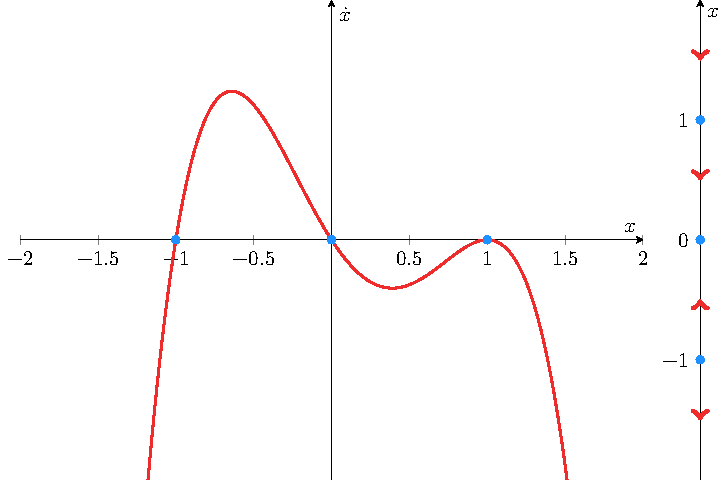
\includegraphics[width = 0.8\linewidth]{figures/phase_line_analysis.pdf}
    \caption{Phase line analysis of the system \(\odv{x}{t} = -x^4 - x^3 - x^2 - x\).
        \(x_e = 1\) is a semi-stable equilibrium point, \(x_e = 0\) is a stable
        equilibrium point, and \(x_e = -1\) is an unstable equilibrium point.}
\end{figure}
The solution to this system is an implicit function:
\begin{equation*}
    g\left( x \right) = x \left( x+1 \right)^{-1/4} \left( x-1 \right)^{-3/4} \exp\left( -\frac{1}{2\left( x-1 \right)} \right) = A e^{-t},
\end{equation*}
where \(A\) solves the initial condition \(x\left( 0 \right) = x_0\):
\begin{equation*}
    A = x_0 \left( x_0 + 1 \right)^{-1/4} \left( x_0 - 1 \right)^{-3/4} \exp\left( -\frac{1}{2\left( x_0 - 1 \right)} \right).
\end{equation*}
\subsection{Solution Curves}
This analysis allows us to construct \textbf{solution curves} for a
system, which are curves in the \(x\)-\(t\) plane that represent the
solution \(x\) as a function of time \(t\). Here we mark equilibrium
points on the vertical axis, and draw trajectories to represent the
possible behaviours of the system around all equilibrium points over
time. A system has \textbf{finite-time blow up} if one of these
trajectories approaches infinity in finite time. This time often
depends on the initial condition. The solution curves for the system
\(\odv{x}{t} = -x^4 - x^3 - x^2 - x\) are shown below:
\begin{figure}[H]
    \centering
    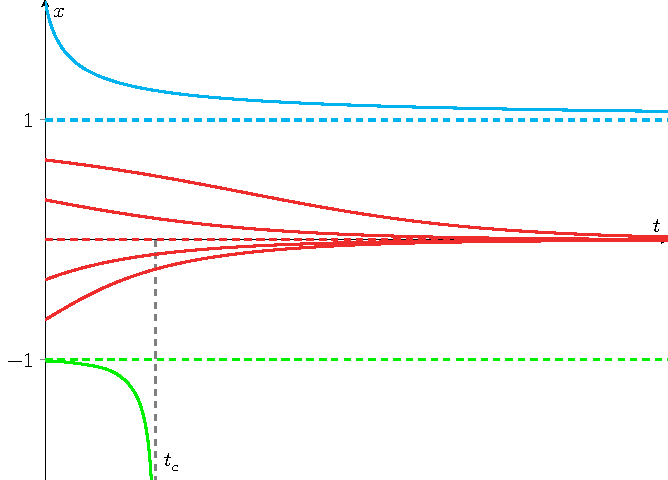
\includegraphics[width = 0.8\linewidth]{figures/solution_curve_analysis.pdf}
    \caption{Solution curves of the system \(\odv{x}{t} = -x^4 - x^3 - x^2 - x\).
        The system experiences finite-time blow up for the time \(t_c\) at which
        \(g\left( x \right)\) is singular.}
\end{figure}
\subsection{Bifurcation Analysis}
Consider a parametrised differential equation of the form:
\begin{equation*}
    \odv{x}{t} = g\left( x,\: \lambda \right).
\end{equation*}
Here we consider the behaviour of the function
\(g\left( x,\: \lambda \right)\) as a function of the parameter
\(\lambda\). We make note of special values of \(\lambda\) at which the
equilibrium points \(x_e\) change, for example, \(\lambda < 0\),
\(\lambda = 0\), and \(\lambda > 0\). This lets us draw a
\textbf{bifurcation diagram} for the system by plotting the contour
\(g\left( x,\: \lambda \right) = 0\) on an \(x\)-\(\lambda\) plane, which shows
how equilibrium points evolve as the parameter \(\lambda\) is varied. We
can depict the stability of these contours by drawing vertical arrows
above and below lines, or by using solid and dashed lines. Here, solid
lines represent stable equilibrium points, while dashed lines represent
unstable equilibrium points.
\subsection{Stability Analysis Example}
Consider the following nonlinear parametrised differential equation:
\begin{equation*}
    \odv{x}{t} = g\left( x,\: \lambda \right) = \lambda x + x^2 - x^3.
\end{equation*}
We can find equilibrium points \(x_e\) by solving:
\begin{equation*}
    \odv{x}{t} = 0 \implies \lambda x + x^2 - x^3 = 0.
\end{equation*}
This gives us three equilibrium points:
\begin{equation*}
    x_{e1} = 0,\: x_{e2} = \frac{1 - \sqrt{1 + 4\lambda}}{2},\: x_{e3} = \frac{1 + \sqrt{1 + 4\lambda}}{2}.
\end{equation*}
To classify the stability of these points, we must consider how the
function \(g\left( x,\: \lambda \right)\) behaves for various values of
\(\lambda\). For this analysis, we will consider the following cases:
\begin{itemize}
    \item \(\lambda < -1/4\): The discriminant \(1 + 4 \lambda\) is
          negative, so the system only has one equilibrium point
          \(x_e = 0\).
    \item \(\lambda = -1/4\): The discriminant \(1 + 4 \lambda\) is
          zero, so the system has two equilibrium points
          \(x_{e1} = 0\) and \(x_{e2} = 1/2\) with multiplicity 2.
    \item \(-1/4 < \lambda < 0\): The discriminant \(1 + 4 \lambda\) is
          positive, and the system has three equilibrium points.
    \item \(\lambda = 0\): The discriminant \(1 + 4 \lambda\) is
          positive, but one of the roots is zero, so the system has two
          equilibrium points \(x_{e1} = 0\) with multiplicity 2 and
          \(x_{e2} = 1/2\).
    \item \(0 < \lambda < 1/4\): The discriminant \(1 + 4 \lambda\) is
          positive, and the system has three equilibrium points.
\end{itemize}
A plot of each of these cases is shown below:
\begin{figure}[H]
    \centering
    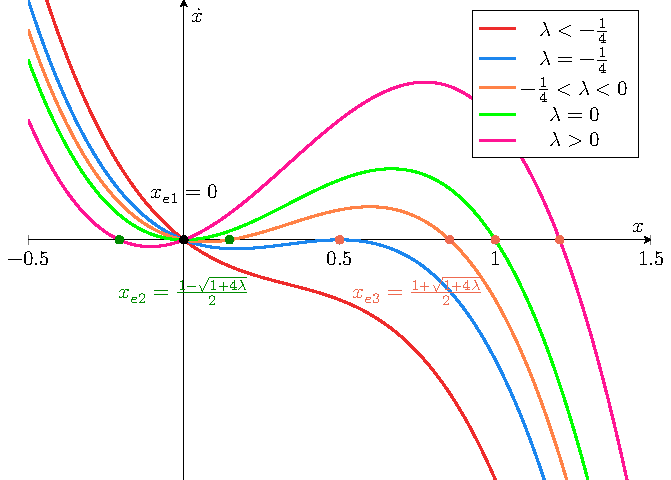
\includegraphics[width=0.8\linewidth]{figures/parametrised_phase_line.pdf}
    \caption{Behaviour of the system \(\odv{x}{t} = \lambda x + x^2 - x^3\) for various values of \(\lambda\).}
\end{figure}
From these plots, we can identify the stability of each region on 5
phase lines or draw these directly onto a bifurcation diagram.
\begin{figure}[H]
    \centering
    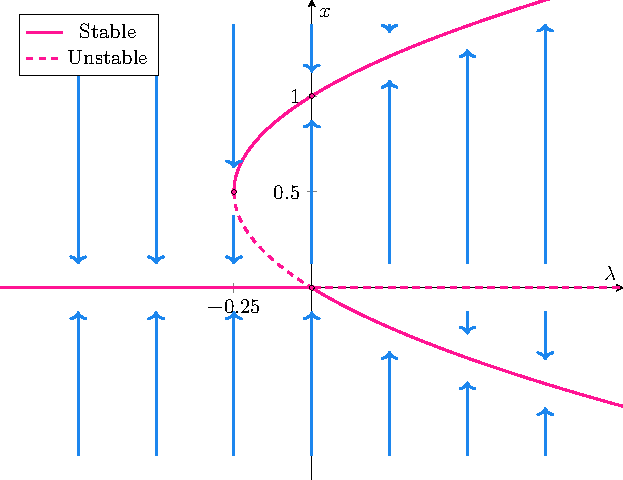
\includegraphics[width = 0.8\linewidth]{figures/bifurcation_diagram.pdf}
    \caption{Bifurcation diagram of the system \(\odv{x}{t} = \lambda x + x^2 - x^3\).} % \label{}
\end{figure}

\section{System of Differential Equations}
Consider a two-dimensional system of differential equations:
\begin{align*}
    \odv{x}{t} & = f\left( x,\: y \right)  \\
    \odv{y}{t} & = g\left( x,\: y \right).
\end{align*}
If we restrict \(f\) and \(g\) to be linear functions of \(x\) and \(y\),
then we can express this as a system of linear equations:
\begin{equation*}
    \odv{\symbf{x}}{t} = \symbf{A} \symbf{x} + \symbf{b}
\end{equation*}
where \(\symbf{x} = \left( x\left( t \right),\: y\left( t \right) \right)\).
As with first-order ODEs, let us first consider the homogeneous part of
this equation and assume the solution form:
\begin{equation*}
    \symbf{x} =
    \begin{bmatrix}
        v_1 e^{\lambda t} \\
        v_2 e^{\lambda t}
    \end{bmatrix}
    = \symbf{v} e^{\lambda t}
\end{equation*}
for constants \(v_i\) and \(\lambda\). If we substitute this back into
the original system, we find the eigenvalue problem:
\begin{align*}
    \odv*{\left( \symbf{v} e^{\lambda t} \right)}{t} & = \symbf{A} \symbf{v} e^{\lambda t} \\
    \lambda \symbf{v} e^{\lambda t}                  & = \symbf{A} \symbf{v} e^{\lambda t} \\
    \symbf{A} \symbf{v}                              & = \lambda \symbf{v}.
\end{align*}
Therefore, by solving for the eigenvalues and eigenvectors of \(\symbf{A}\),
we can determine the general solution to this system of differential
equations.
\subsection{Real Distinct Eigenvalues}
If the eigenvalues of \(\symbf{A}\) are real and distinct, then the
general solution to the system of differential equations is given by:
\begin{equation*}
    \symbf{x} = c_1 \symbf{v}_1 e^{\lambda_1 t} + c_2 \symbf{v}_2 e^{\lambda_2 t}
\end{equation*}
where \(\symbf{v}_1\) and \(\symbf{v}_2\) are the eigenvectors of
\(\symbf{A}\) corresponding to the eigenvalues \(\lambda_1\) and
\(\lambda_2\), and \(c_1\) and \(c_2\) are constants determined by the
initial conditions.
\begin{itemize}
    \item When \(\lambda_1, \lambda_2 < 0\), the system has a
          \textbf{stable node} at the origin. The trajectories of the
          system approach this node as \(t \to \infty\).
    \item When \(\lambda_1, \lambda_2 > 0\) with \(\lambda_1 >
          \lambda_2\), the system has an \textbf{unstable node} at the
          origin. In general \(\symbf{x} \sim c_1 \symbf{v}_1
          e^{\lambda_1 t}\) as \(t \to \infty\).
    \item When \(\lambda_1 < 0 < \lambda_2\), the system has a
          \textbf{saddle point} at the origin. In general, \(\symbf{x}
          \sim c_2 \symbf{v}_2 e^{\lambda_2 t}\) as \(t \to \infty\),
          but certain initial conditions can cause trajectories to
          approach the origin.
\end{itemize}
\subsection{Real Repeated Eigenvalues}
If the eigenvalues of \(\symbf{A}\) are real and repeated, then the
general solution to the system of differential equations depends on the
number of linearly independent eigenvectors corresponding to the
repeated eigenvalue \(\lambda\):
\begin{itemize}
    \item If the system has two linearly independent eigenvectors
          \(\symbf{v}_1\) and \(\symbf{v}_2\), then the general
          solution is given by:
          \begin{equation*}
              \symbf{x} = c_1 \symbf{v}_1 e^{\lambda t} + c_2 \symbf{v}_2 e^{\lambda t}.
          \end{equation*}
    \item If the system has only one linearly independent eigenvector
          \(\symbf{v}\), then the general solution is given by:
          \begin{equation*}
              \symbf{x} = c_1 \symbf{v} e^{\lambda t} + c_2 \left( \symbf{v} t + \symbf{w}  \right) e^{\lambda t}
          \end{equation*}
          where \(\symbf{w}\) is a generalised eigenvector that
          satisfies:
          \begin{equation*}
              \left( \symbf{A} - \lambda \symbf{I} \right) \symbf{w} = \symbf{v}.
          \end{equation*}
\end{itemize}
In both cases, the system has a \textbf{degenerate node} at the origin:
\begin{itemize}
    \item When \(\lambda < 0\), we have a \textbf{degenerate stable
          node} at the origin. Trajectories of the system move towards
          the origin.
    \item When \(\lambda > 0\), we have a \textbf{degenerate unstable
          node} at the origin. Trajectories of the system move away
          from the origin.
\end{itemize}
\subsection{Complex Eigenvalues}
If the eigenvalues of \(\symbf{A}\) are complex, then the general
solution to the system of differential equations is given by:
\begin{equation*}
    \symbf{x} = c_1 \left[ \symbf{w}_1 \cos\left( \beta t \right) - \symbf{w}_2 \sin\left( \beta t \right) \right] e^{\alpha t} + c_2 \left[ \symbf{w}_2 \cos\left( \beta t \right) + \symbf{w}_1 \sin\left( \beta t \right) \right] e^{\alpha t}
\end{equation*}
where \(\alpha\) and \(\beta\) are the real and imaginary parts of the
complex eigenvalues \(\lambda = \alpha \pm i \beta\), with corresponding
eigenvectors \(\symbf{v}_1\) and \(\symbf{v}_2\), which we have used to
defined \(\symbf{w}_1 = \left( \symbf{v}_1 + \symbf{v}_2 \right) / 2\)
and \(\symbf{w}_2 = \left( \symbf{v}_1 - \symbf{v}_2 \right) / 2i\).
\begin{itemize}
    \item When \(\alpha < 0\), the system has a \textbf{stable spiral}
          (source) at the origin and trajectories of the system spiral
          inwards towards. In this case, the solution oscillates and
          decays as \(t \to \infty\).
    \item When \(\alpha > 0\), the system has an \textbf{unstable
          spiral} (sink) at the origin and trajectories of the system
          spiral outwards. In this case, the solution oscillates and
          grows exponentially as \(t \to \infty\).
    \item When \(\alpha = 0\), the system has a \textbf{centre} at the
          origin and trajectories of the system spiral around the
          origin without growth or decay. In this case, the solution
          oscillates indefinitely.
\end{itemize}
The orientation of this spiral is determined by finding the direction of
the system near the origin by evaluating \(\symbf{A} \symbf{x}_0\)
for some small vector \(\symbf{x}_0\).
\subsection{Nonlinear Systems}
As in the case of a single nonlinear differential equation, we can use
qualitative methods to understand the behaviour of solutions to a
nonlinear system of differential equations. Consider the
two-dimensional system of differential equations introduced earlier:
\begin{align*}
    \odv{x}{t} & = f\left( x,\: y \right)  \\
    \odv{y}{t} & = g\left( x,\: y \right).
\end{align*}
Equilibrium points for this system are defined as points \(\left( x_e,\: y_e \right)\)
that satisfy \(f\left( x_e,\: y_e \right) = 0\) and \(g\left( x_e,\: y_e \right) = 0\).
If we consider the small region around an equilibrium point
\(\left( x_e,\: y_e \right)\), we can analyse the local behaviour of
the system by linearising the system about this point. This involves
using a first-order Taylor series approximation of the system near the
equilibrium point:
\begin{align*}
    f\left( x,\: y \right) & \approx f\left( x_e,\: y_e \right) + \pdv{f}{x}\left( x - x_e \right) + \pdv{f}{y}\left( y - y_e \right)  \\
    g\left( x,\: y \right) & \approx g\left( x_e,\: y_e \right) + \pdv{g}{x}\left( x - x_e \right) + \pdv{g}{y}\left( y - y_e \right).
\end{align*}
Substituting this back into the system, we obtain the linearised system:
\begin{equation*}
    \odv*{
        \begin{bmatrix}
            x - x_e \\
            y - y_e
        \end{bmatrix}
    }{t} =
    \begin{bmatrix}
        \displaystyle \pdv{f}{x} & \displaystyle \pdv{f}{y} \\[2ex]
        \displaystyle \pdv{g}{x} & \displaystyle \pdv{g}{y}
    \end{bmatrix}
    _{\left( x_e,\: y_e \right)}
    \begin{bmatrix}
        x - x_e \\
        y - y_e
    \end{bmatrix}
    \iff \odv*{\left( \symbf{x} - \symbf{x}_e \right)}{t} = \symbf{J} \left( \symbf{x} - \symbf{x}_e \right)
\end{equation*}
where \(\symbf{J}\) is the Jacobian matrix of the system evaluated at
the equilibrium point \(\left( x_e,\: y_e \right)\). We can then find
the local behaviour of the system by finding the eigenvalues of
\(\symbf{J}\) for each equilibrium point.
\subsection{Phase Plane Analysis}
Using the above information, we can draw a \textbf{phase plane} to
visualise the behaviour of the system over time. Here the horizontal
axis represents the change in \(x\) and the vertical axis represents
the change in \(y\). We mark equilibrium points on the phase plane and
draw eigenvectors from these points to represent the trajectory of the
system near equilibrium points. The direction of trajectories along
eigenvectors is determined by the sign of the corresponding
eigenvalues.

We can also draw \textbf{nullclines} on the phase plane, which are
curves where one of \(f\) or \(g\) is equal to zero.
\end{document}
